
\section{Closing the loop}

%% rolling experiment

Poking is sufficient to explore some very simple affordances of
objects, such as rolling, toppling, breaking etc.  We explore the
rolling affordance with the four objects shown in
Figure~\ref{fig:rolling-motivate}.  Each of the objects rolls in a
different way, which the robot can learn about and exploit.

\begin{figure}[tbh]
  \centerline{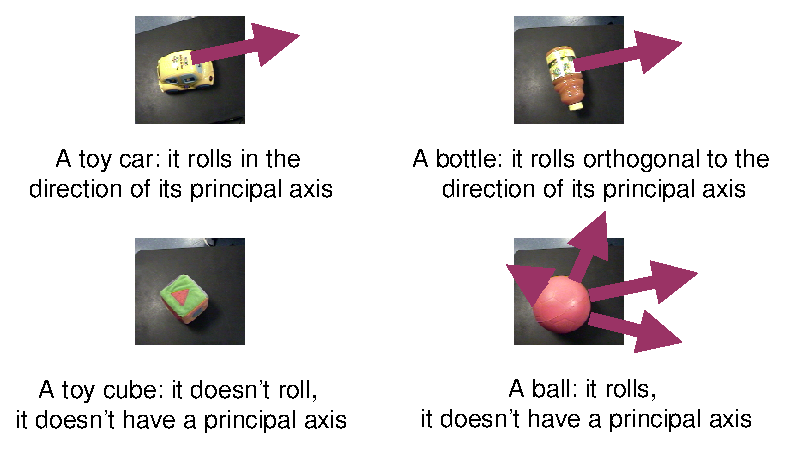
\includegraphics[width=12cm]{rolling-motivate}}
  \caption{
%
    Different objects roll in different ways.  A toy car rolls
    forward, a bottle rolls on its side, a sphere rolls in any
    direction, and a cube doesn't really roll at all.
%
} 
  \label{fig:rolling-motivate}
\end{figure}

\begin{figure}[tbh]
  \centerline{\includegraphics[width=12cm]{rolling-graphs}}
  \caption{
%
  The robot relates the direction an object moves in with the
  direction of its principal axis.  For a car, there is a clear
  tendency to roll in the direction of the principal axis.
  A bottle has a clear tendency to roll towards its side.
  Cars and spheres have no clear principal axis so, whether they
  roll or not, there is nothing to say.
%
} 
  \label{fig:rolling-graphs}
\end{figure}

The final behavior of the robot after training is: human presents an
object, makes it roll.  Presents the same object, perhaps in another
orientation, and the robot pushes it in the right direction to make it
roll.  If the human hits the object in a non-canonical direction,
so will the robot.  This serves to demonstrate the full loop of 
perception and action.



